\documentclass[11pt]{article}

\usepackage[scale=1]{ccicons}
\usepackage{metalogo}
\usepackage{xcolor,colortbl}
\usepackage{multicol,multirow,booktabs}
\usepackage{graphicx}
\usepackage{bm}
\usepackage{fontawesome5}
\usepackage{xsim}
% Definir un nuevo tipo de ejercicio llamado "Pregunta"
\DeclareExerciseType{pregunta}{
  exercise-env = pregunta,
  solution-env = respuesta,
  exercise-name = Pregunta,
  solution-name = Respuesta,
  exercise-template = simple,
  solution-template = simple,
}

\usepackage[paper=a4paper, headheight=110pt,showframe=false, 
            layoutvoffset=2em,
            bottom=2cm, top=3.5cm, left=2.5cm, right=2.0cm]{geometry}
\usepackage[spanish, es-nodecimaldot]{babel}
\DeclareExerciseTranslations{exercise}{
  Fallback = exercise,
  English = exercise,
  Spanish = ejercicio
}
\usepackage{hyperref}
\usepackage{amsmath}
\usepackage{mismath}
\usepackage{gensymb,amssymb}
\setlength{\parindent}{3em}
\setlength{\parskip}{1em} 
\usepackage[shortlabels]{enumitem}
\usepackage{subcaption}
\usepackage{wrapfig}
\usepackage{siunitx}
%\usepackage{mathspec}
%\usepackage{unicode-math}


% Fonts can be customized here.
\defaultfontfeatures{Mapping=tex-text}
\setmainfont [Ligatures={Common}]{Linux Libertine O}
\setmonofont[Scale=0.9]{Linux Libertine Mono O}
%\usepackage[svgnames]{xcolor} % Gestión de colores
\usepackage{hyperref}
\hypersetup{
  colorlinks=true, linktocpage=true, pdfstartpage=3, pdfstartview=FitV,%
  breaklinks=true, pageanchor=true,%
  pdfpagemode=UseNone, %
  plainpages=false, bookmarksnumbered, bookmarksopen=true, bookmarksopenlevel=1,%
  hypertexnames=true, pdfhighlight=/O,%nesting=true,%frenchlinks,%
  urlcolor=Maroon, linkcolor=RoyalBlue, citecolor=Blue, %pagecolor=RoyalBlue,%
  pdftitle={},%
  pdfauthor={\textcopyright\ C. Manuel Carlevaro},%
  pdfsubject={},%
  pdfkeywords={},%
  pdfcreator={XeLaTeX},%
  pdfproducer={XeLaTeX}%
}

%% Operadores
\DeclareMathOperator{\sen}{sen}
\DeclareMathOperator{\senc}{senc}
\DeclareMathOperator{\sign}{sign}
\newcommand{\T}[1]{\underline{\bm{#1}}}
\DeclareMathOperator{\Tr}{Tr}
%\NewDocumentCommand{\evalat}{sO{\big}mm}{%
  %\IfBooleanTF{#1}
   %{\mleft. #3 \mright|_{#4}}
   %{#3#2|_{#4}}%
%}

\xsimsetup{
solution/print = true
%solution/print = false
}

\title{Introducción a la física}
\author{Manuel Carlevaro}
\date{Universidad de Navarra}


\begin{document}
%\maketitle

\begin{center}
\framebox[1.0\textwidth][c]{
\huge{\textsc{Introducción a la física}} 
}
\end{center} 

\begin{center}
\vspace{1em}
\Large{\textsc{Universidad de Navarra}} 
\end{center}

 \vspace{1em}

\begin{center}
\begin{tabular}{r l}
 \textbf{Tema:} & Trabajo y energía.\\
 \textbf{Profesor:} & Manuel Carlevaro \\
 \textbf{Ayudante:} & Alba Meneses Felipe
\end{tabular}\end{center}

\vspace{2em}

\begin{exercise}
    El signo de muchas cantidades físicas depende de la elección de las coordenadas. Por ejemplo, el valor de $g$ puede ser negativo o positivo, según si elegimos como positiva la dirección hacia arriba o hacia abajo. ¿Lo mismo es válido para el trabajo? En otras palabras, ¿podemos hacer negativo el trabajo positivo con una elección diferente de las coordenadas? Explique su respuesta.
\end{exercise}

\begin{exercise}
    Un elevador es subido por sus cables con rapidez constante. ¿El trabajo realizado sobre él es positivo, negativo o cero? Explique.
\end{exercise}

\begin{multicols}{2}
\begin{exercise}
    En los casos que se muestran en la figura, el objeto se suelta desde el reposo en la parte superior y no sufre fricción ni resistencia del aire. ¿En cuál situación, si acaso, la masa tendrá i) la mayor rapidez al llegar a la parte inferior y ii) el mayor trabajo efectuado sobre ella en el tiempo que tarda en llegar a la parte inferior?
\begin{center}
    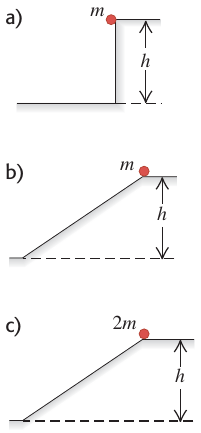
\includegraphics[scale=0.5]{figs/p-01.png}
\end{center}
\end{exercise}
\end{multicols}

\begin{exercise}
    ¿La energía cinética de un automóvil cambia más al acelerar de \num{10} a \qty{15}{m/s} o de \num{15} a \qty{20}{m/s}? Explique su respuesta.
\end{exercise}

\begin{exercise}
Imagine que usted sostiene un portafolios por el asa, con el brazo recto a su costado. ¿La fuerza que la mano ejerce efectúa trabajo sobre el portafolios a) cuando usted camina con rapidez constante por un pasillo horizontal y b) cuando usa una escalera eléctrica para subir del primer al segundo piso de un edificio? Justifique su respuesta en cada caso.
\end{exercise}

\begin{multicols}{2}
\begin{exercise}
    Dos bloques están conectados por un cordón muy ligero que pasa por una polea sin masa y sin fricción (ver figura). Al viajar a rapidez constante, el bloque de \qty{20.0}{N} se mueve \qty{75.0}{cm} a la derecha y el bloque de \qty{12.0}{N} se mueve \qty{75.0}{cm} hacia abajo. Durante este proceso, ¿cuánto trabajo efectúa a) sobre el bloque de \qty{12.0}{N}, i) la gravedad y ii) la tensión en el cordón? b) sobre el bloque de \qty{20.0}{N}, i) la gravedad, ii) la tensión en el cordón, iii) la fricción y iv) la fuerza normal? c) Obtenga el trabajo total efectuado sobre cada bloque.
\begin{center}
    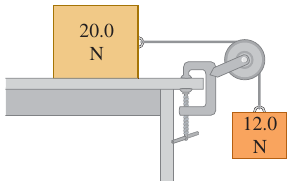
\includegraphics[scale=0.5]{figs/p-02.png}
\end{center}
\end{exercise}
\begin{solution}
    a) (i) \qty{9.00}{J}, (ii) \qty{-9}{J}. b) (i) \num{0}, (ii) \qty{9.00}{J}, (iii) \qty{-9.00}{J}, (iv) \num{0}. c) Cero para cada bloque.
\end{solution}
\end{multicols}

\begin{multicols}{2}
\begin{exercise}
    Alguien empuja horizontalmente una caja de \qty{30.0}{kg} una distancia de \qty{4.5}{m} en un piso plano, con velocidad constante. El coeficiente de fricción cinética entre el piso y la caja es de \num{0.25}. a) ¿Qué magnitud de fuerza debe aplicar el obrero? b) ¿Cuánto trabajo efectúa dicha fuerza sobre la caja? c) ¿Cuánto trabajo efectúa la fricción sobre la caja? d) ¿Cuánto trabajo realiza la fuerza normal sobre la caja? ¿Y la gravedad? e) ¿Qué trabajo total se efectúa sobre la caja?
\end{exercise}
\begin{solution}
    a) \qty{74}{N}, b) \qty{330}{J}, c) \qty{-330}{J}, d) cero, cero, e) cero.
\end{solution}
\end{multicols}

\begin{exercise}
    Una sandía de \qty{4.80}{kg} se deja caer (rapidez inicial cero) desde la azotea de un edificio de \qty{25.0}{m} y no sufre resistencia del aire apreciable. a) Calcule el trabajo realizado por la gravedad sobre la sandía durante su desplazamiento desde la azotea hasta el suelo. b) Justo antes de estrellarse contra el suelo, ¿cuáles son i) la energía cinética y ii) la rapidez de la sandía? c) ¿Cuál de las respuestas en los incisos a) y b) sería diferente si hubiera resistencia del aire considerable?
\end{exercise}

\begin{exercise}
    Se lanza una piedra de \qty{20}{N} verticalmente hacia arriba desde el suelo. Se observa que, cuando está \qty{15.0}{m} sobre el suelo, viaja a \qty{25.0}{m/s} hacia arriba. Use el teorema trabajo-energía para determinar a) su rapidez en el momento de ser lanzada y b) su altura máxima.
\end{exercise}

\begin{multicols}{2}
\begin{exercise}
    Un trineo con masa de \qty{8.00}{kg} se mueve en línea recta sobre una superficie horizontal sin fricción. En cierto punto, su rapidez es de \qty{4.00}{m/s}; \qty{2.50}{m} más adelante, su rapidez es de \qty{6.00}{m/s}. Use el teorema trabajo-energía para determinar la fuerza que actúa sobre el trineo, suponiendo que tal fuerza es constante y actúa en la dirección del movimiento del trineo.
\end{exercise}
\begin{solution}
    \qty{32}{N}.
\end{solution}
\end{multicols}

\begin{multicols}{2}
\begin{exercise}
    A un automóvil a escala de \qty{2.0}{kg}, controlado por radio, se aplica una fuerza $\vec{F}$ paralela al eje $x$; mientras el auto se mueve por una pista recta. La componente $x$ de la fuerza varía con la coordenada $x$ del auto, como se indica en la figura. Calcule el trabajo efectuado por la fuerza $\vec{F}$ cuando el auto se mueve de a) $x = 0$ a $x = \qty{3.0}{m}$; b) $x = \qty{3.0}{m}$ a $x = \qty{4.0}{m}$; c) $x = 4$ a $x = \qty{7.0}{m}$; d) $x = 0$ a $x = \qty{7.0}{m}$; e) $x = \qty{7.0}{m}$ a $x = \qty{2.0}{m}$.
\begin{center}
    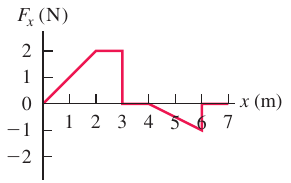
\includegraphics[scale=0.5]{figs/p-03.png}
\end{center}
\end{exercise}
\begin{solution}
a) \qty{4.0}{J}; b) cero; c) \qty{-1.0}{J}; d) \qty{3.0}{J}; e) \qty{-1.0}{J}.
\end{solution}
\end{multicols}

\begin{exercise}
Suponga que el auto del problema anterior está inicialmente en reposo en $x = 0$ y que $\vec{F}$ es la fuerza neta que actúa sobre él. Use el teorema trabajo-energía para determinar la rapidez del auto en a) $x = \qty{3.0}{m}$; b) $x = \qty{4.0}{m}$; c) $x = \qty{7.0}{m}$.
\end{exercise}

\begin{exercise}
    Una piedra de \qty{20.0}{kg} se desliza por una superficie horizontal áspera a \qty{8.0}{m/s} y finalmente se para debido a la fricción. El coeficiente de fricción cinética entre la piedra y la superficie es de \num{0.200}. ¿Cuánta potencia térmica media se produce al detenerse la piedra?
\end{exercise}

\begin{multicols}{2}
\begin{exercise}
    Una caja de \qty{6.0}{kg} que se mueve a \qty{3.0}{m/s}, sobre una superficie horizontal sin fricción, choca con un resorte ligero cuya constante de fuerza es de \qty{75}{N/cm}. Use el teorema trabajo-energía para determinar la compresión máxima del resorte.
\end{exercise}
\begin{solution}
    \qty{8.5}{cm}.
\end{solution}
\end{multicols}

\begin{multicols}{2}
\begin{exercise}
    Un equipo de dos personas en una bicicleta tándem debe vencer una fuerza de \qty{165}{N} para omantener una rapidez de \qty{9.00}{m/s}. Calcule la potencia requerida por ciclista, suponiendo contribuciones iguales. Exprese su respuesta en watts y en caballos de potencia.
\end{exercise}
\begin{solution}
    \qty{743}{W}, \qty{0.995}{hp}.
\end{solution}
\end{multicols}

\begin{exercise}
    Un elevador vacío tiene masa de \qty{600}{kg} y está diseñado para subir con rapidez constante una distancia vertical de \qty{20.0}{m} (5 pisos) en \qty{16.0}{s}. Es impulsado por un motor capaz de suministrar \qty{40}{hp} al elevador. ¿Cuántos pasajeros como máximo pueden subir en el elevador? Suponga una masa de \qty{65.0}{kg} por pasajero.
\end{exercise}

\begin{exercise}
    El consumo total de energía eléctrica en Estados Unidos es del orden de \qty{1e19}{J} por año. a) ¿Cuál es la tasa media de consumo de energía eléctrica en watts? b) Si la población de ese país es de 300 millones de personas, determine la tasa media de consumo de energía eléctrica por persona. c) El Sol transfiere energía a la Tierra por radiación a razón de \qty{1.0}{kW} por \unit{m^2} de superficie, aproximadamente. Si esta energía pudiera recolectarse y convertirse en energía eléctrica con eficiencia del 40\%, ¿qué área (en \unit{km^2}) se requeriría para recolectar la energía eléctrica gastada por Estados Unidos?
\end{exercise}


\end{document}
